%%%%%%%%%%%%%%%%%%%%%%%%%%%%%%%%%%%%%%%%%%%%%%%%%%%%%%%%%%%%%%%%%%%%%%%%%%%%%%%%
% data_set.tex:
%%%%%%%%%%%%%%%%%%%%%%%%%%%%%%%%%%%%%%%%%%%%%%%%%%%%%%%%%%%%%%%%%%%%%%%%%%%%%%%%
\chapter{Background Estimation}
\label{sec:backgroundEstimation}
%%%%%%%%%%%%%%%%%%%%%%%%%%%%%%%%%%%%%%%%%%%%%%%%%%%%%%%%%%%%%%%%%%%%%%%%%%%%%%%%
The event selection described in Chapter \ref{sec:event_selection_chapter} was developed for high 
sensitivity to a \WR boson signal.  However, when this selection was applied to data, events from 
Standard Model (SM) processes were selected.  The number of events expected in data from SM processes 
was estimated using simulated \MC datasets listed in Chapter \ref{sec:event_selection_chapter}.  
The procedures used to calculate and validate the expected SM backgrounds are described here.

\section{Top Quark Background}
\label{sec:topQrkBkgnds}
SM processes that produced one or more top quarks constituted one of the two largest backgrounds 
to the \WR and \nul search in the $\ell\ell jj$ final state.  Based on cross sections times branching 
fractions to $\ell\ell jj$ final states listed in Chapter \ref{sec:MC}, production 
of top-anti top quark pairs ($\ttbar$, Figure \ref{fig:ttbarDiag}) and single top quarks in association 
with W bosons (top+W, Figure \ref{fig:singleTopDiags}) contributed the majority of top quark events that passed 
the full event selection.  In such processes, nearly 100\% of top quarks decayed to a bottom quark 
and SM W boson, and the W boson was free to decay to any charged lepton.  One consequence of this freedom 
was that $\ttbar$ and top+W production yielded the $e\mu jj$ final state approximately twice as often 
as the $eejj$ or $\mu\mu jj$ final states.  This consequence was instrumental in estimating the top quark 
background.

\begin{figure}[h]
	\centering
	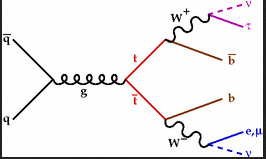
\includegraphics[width=0.7\textwidth]{figures/topAntiTopFeynDiagram.png}
	\caption{$\ttbar$ Feynman diagram \cite{ttbarDiagram}.}
	\label{fig:ttbarDiag}
\end{figure}

\begin{figure}[h]
	\centering
	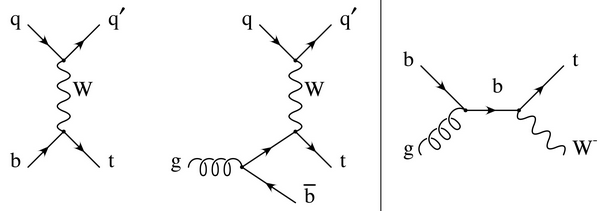
\includegraphics[width=0.7\textwidth]{figures/singleTopQuarkFeynDiagrams.png}
	\caption{Single top quark Feynman diagrams \cite{singleTopQrkDiagrams}.}
	\label{fig:singleTopDiags}
\end{figure}

The top quark background was estimated directly from collision data that passed the $e\mu$ channel requirements.  
An estimate of the pure top quark background was possible in the $e\mu$ channel for several reasons.  Based on 
the lepton flavor conservation assumption stated in Chapter \ref{sec:lrsPhenomenology}, a \WR signal produced 
events that passed the $e\mu$ channel selections at a rate suppressed by the weak coupling constant 
$g_{R} \sim \frac{1}{100}$.  In addition, the SM backgrounds without top quarks listed in Chapter \ref{sec:MC} 
produced events that passed the $e\mu$ channel selection at a rate suppressed by the electromagnetic coupling 
constant $\alpha \sim \frac{1}{100}$.  Thus, the $e\mu$ channel was expected to be dominated by top quark 
processes.  This was confirmed by comparing $e\mu$ channel data and simulations, as shown in Figure \ref{fig:dataAndSimsInEMuChannel}.

\begin{figure}[h]
	\centering
	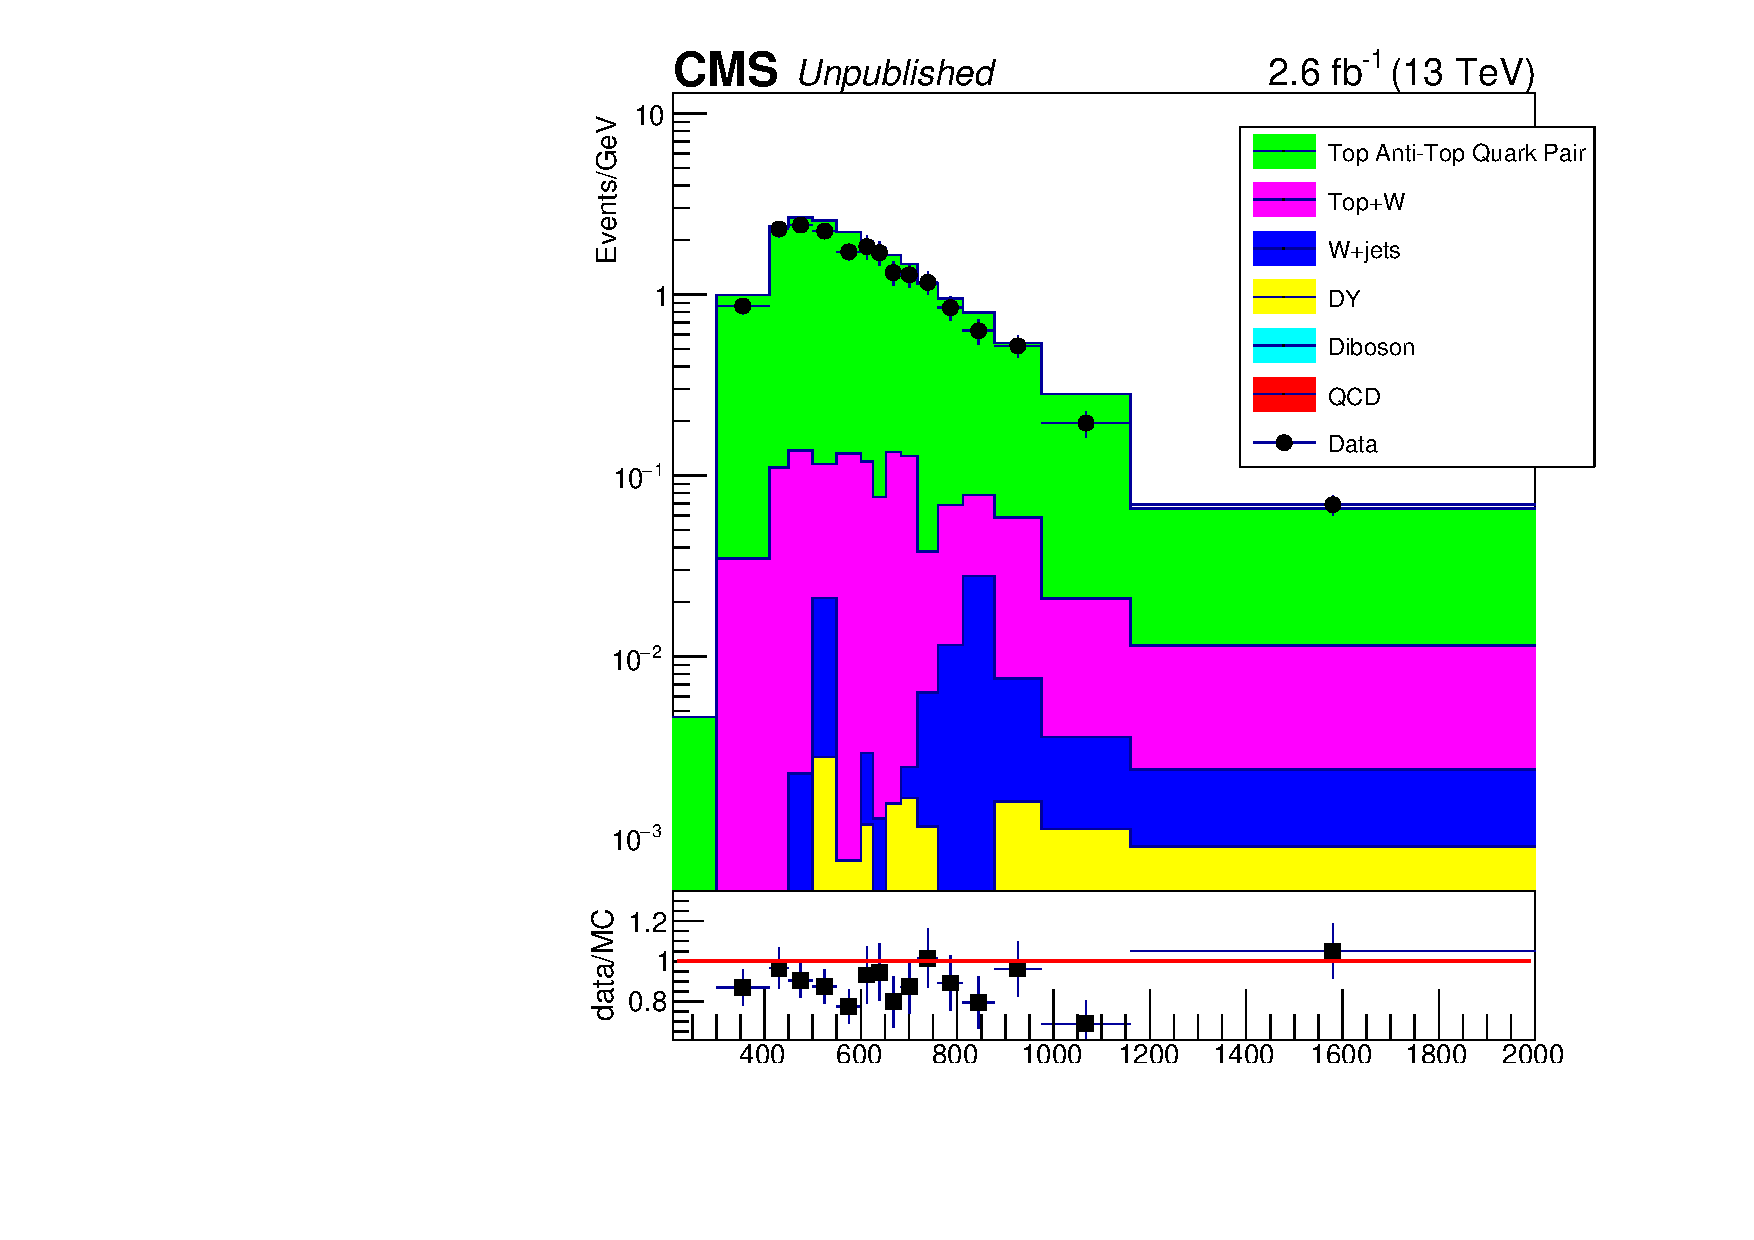
\includegraphics[width=0.7\textwidth]{figures/Mlljj_eMuChannel_log.pdf}
	\caption{The $\Mlljj$ distribution from data and simulated SM events that passed the $e\mu$ selection, excluding 
	the $\Mlljj > 600 \GeV$ cut.  The bin widths are variable, and their contents are normalized to the bin widths.}
	\label{fig:dataAndSimsInEMuChannel}
\end{figure}

To estimate the top quark background in the $eejj$ and $\mu\mu jj$ signal regions, scale factors (SFs) were 
calculated that scaled $e\mu jj$ data events into $eejj$ and $\mu\mu jj$ events.  The SFs were calculated using 
simulated top quark events and the following procedure:

\begin{itemize}
	\item Simulated top quark events were selected using the $ee$, $e\mu$, and $\mu\mu$ channel requirements.
	\item Using selected events, the \Meejj, \Memujj and \Mmumujj distributions were produced.
	\item Using the integrals \Nemujj and \Nlljj of the \Memujj and \Mlljj distributions, the top quark background SF 
		for the $\ell\ell jj$ final state was calculated as $\Nlljj / \Nemujj$.
\end{itemize}

The SF was $0.432$ in the $ee$ channel and $0.659$ in the $\mu\mu$ channel.  The $ee$ ($\mu\mu$) channel SF 
was below (above) the expected SF of $0.5$ because electrons were reconstructed with a reduced $|\eta|$ acceptance, 
and selected with a lower efficiency identification selection relative to muons.  The number of simulated top quark 
events used to calculate the SFs decreased rapidly with increasing \Mlljj, so the SFs were determined primarily by 
simulated events with $\Mlljj < 1500\GeV$.  Using SFs that did not vary with \Mlljj created an uncertainty in the 
top quark background estimate proportional to the fluctuations of \Mmumujj/\Memujj and \Meejj/\Memujj around the 
constant SFs versus \Mlljj in Figure \ref{fig:ttbarSFratios}.  This uncertainty was covered by assigning a 10\% 
uncertainty to both SFs.

After calculating the SFs, the top quark background in the $\mu\mu jj$ ($eejj$) final state was estimated by 
multiplying the \Memujj distribution from data by $0.659$ ($0.432$).  Contributions of non-top quark backgrounds 
in the $e\mu$ channel were more than one order of magnitude smaller than the 10\% top quark background uncertainty, 
so no events were subtracted from $e\mu$ channel data to account for non-top quark backgrounds.

\begin{figure}[h]
\centering
\subfigure[][Ratio of \Meejj and \Memujj]{
  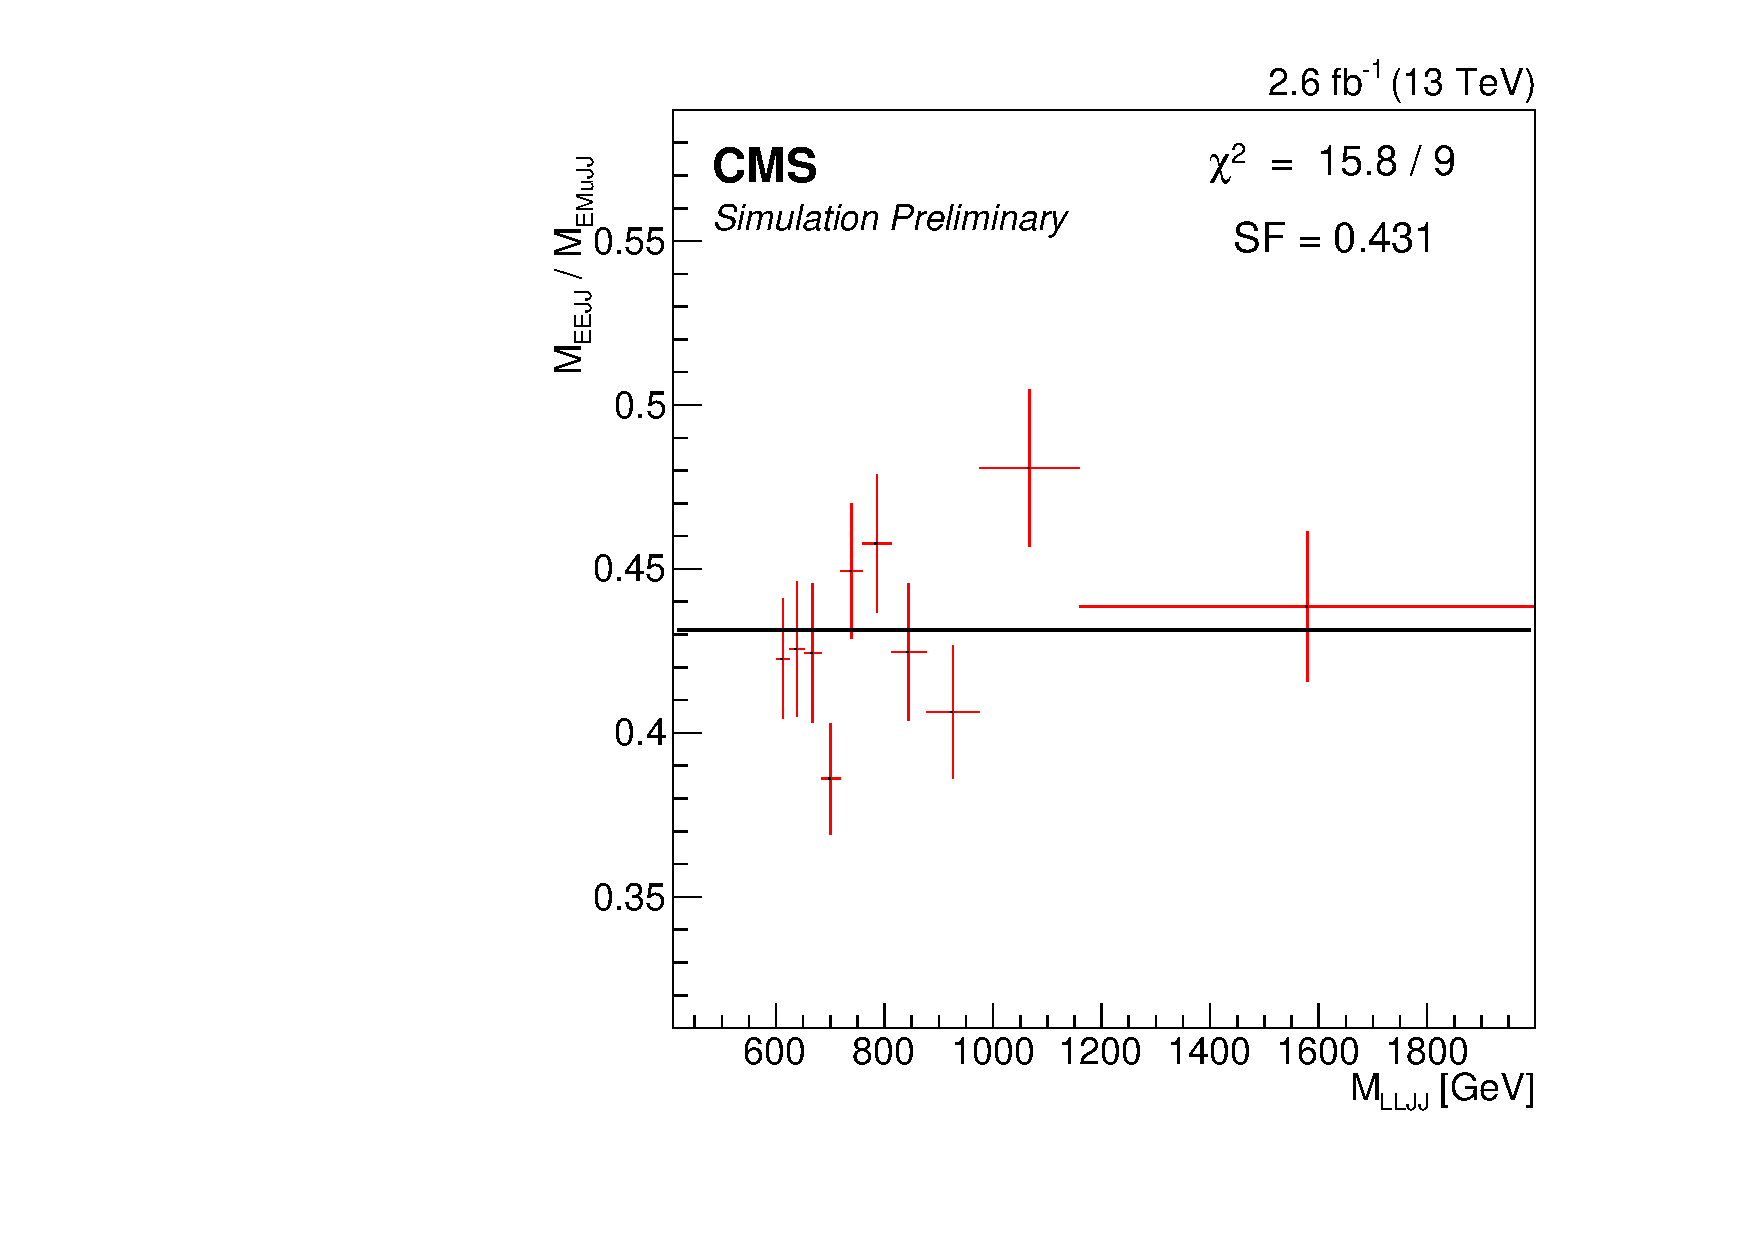
\includegraphics[width=0.50\textwidth]{figures/flavor_ratio_EE_variablebinwidth.pdf}
}
\subfigure[][Ratio of \Mmumujj and \Memujj]{
  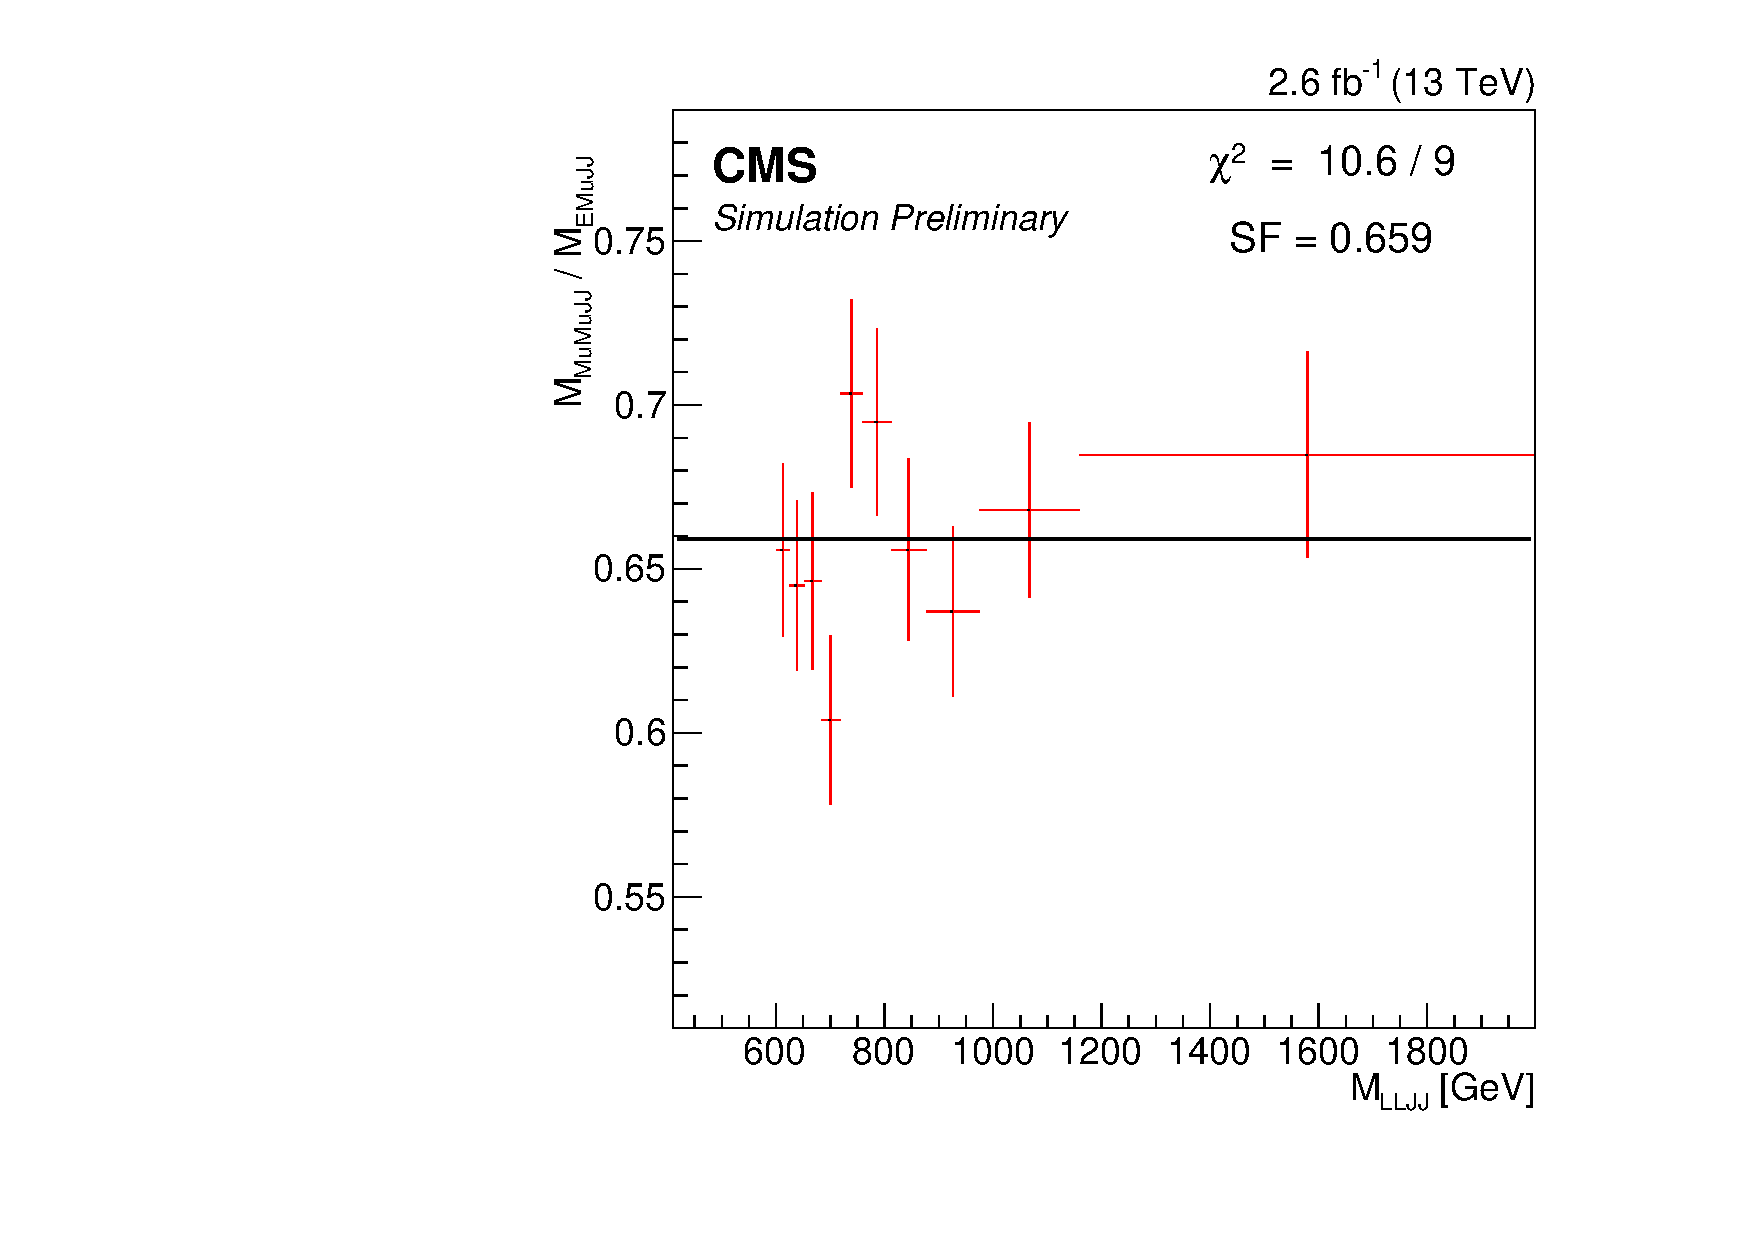
\includegraphics[width=0.50\textwidth]{figures/flavor_ratio_MuMu_variablebinwidth.pdf}
}
\caption{Bin-by-bin ratio of \Mlljj distribution and \Memujj from simulated top quark backgrounds, where $\ell$ was an electron (left) or a muon (right). }
\label{fig:ttbarSFratios}
\end{figure}


\section{\DY Background}
\label{sec:dyBkgnd}
The production and decay of Z bosons to lepton pairs with jets ($\DY$+jets), $pp \rightarrow Z+jets \rightarrow \ell\ell+jets$, 
was the other of the two largest backgrounds to the \WR and \nul search in the $\ell\ell jj$ final state.  The \DY 
background was estimated using simulated $\DY$+jets events.  Mis-modelling of $\DY$+jets in simulations lead to two discrepancies 
with respect to data, and their sizes were estimated in two control regions.

The first discrepancy was a difference in normalization between data and \MC, caused by the cross section uncertainty in 
the simulation.  The size of the discrepancy was estimated by comparing $Z \rightarrow \ell\ell$ events in data and 
\DY simulations, selected with the following requirements:

\begin{itemize}
	\item One of the background only triggers described in Chapter \ref{sec:triggers} was fired.
	\item At least two leptons were found with $\pt > 35 \GeV$ that passed identification cuts described in 
		Chapter \ref{sec:event_selection_chapter}.  If more than two leptons were found, only the two highest $\pt$ 
		leptons were used.
	\item At least two jets were found with $\pt > 40 \GeV$ that passed identification cuts.  If more than two jets 
		were found, only the two highest $\pt$ jets were used.
	\item The leptons and jets had $|\eta| < 2.4$.
	\item The two leptons had di-lepton mass $70 < M_{\ell\ell} < 110 \GeV$.
	\item Both leptons were separated from both jets by $\Delta R > 0.4$.
\end{itemize}

Using selected events, the $\Mll$ distribution was made and used to compare data to simulations.  Based on simulations 
of non-\DY backgrounds, 3\% of the selected events in data came from non-\DY processes.  The effect of subtracting 
simulated non-\DY events from data was much smaller than an independent uncertainty assigned to the \DY background 
estimate, so non-\DY backgrounds were not subtracted from data.  The normalization of the $\Mll$ distribution using 
data events exceeded that of simulated events by 15.7\% in the $ee$ channel, and 14.2\% in the $\mu\mu$ channel.  To 
correct the normalization discrepancy, the \DY background estimate derived from simulated events in the signal and 
other control region was scaled up by the appropriate percentage.

Two additional $\DY$+jets simulated datasets using different generators for the first simulation step were used to 
estimate an uncertainty on the $\sim$15\% correction to the \DY background predicted by simulations.  The $Z \rightarrow \ell\ell$ 
selection described earlier without jet requirements was applied to data and all three simulated $\DY$+jets datasets.  
The jet requirements were removed to compare data to simulations in a phase space where all three simulated datasets 
yielded a large number of selected events.  Using selected events, the normalization discrepancy between data and 
simulations in the $\Mll$ distribution was calculated, and the largest discrepancy was taken as a systematic 
uncertainty on $\sim$15\%.  This uncertainty was estimated to be 2.0\% (1.0\%) in the $ee$ ($\mu\mu$) channel.

After.

The selections described in Chapter \ref{sec:event_selection_chapter} 
were applied to simulated events, and the selected events represented the \DY background estimate.  However, mis-modelling 
of $\DY$+jets in simulations lead to two discrepancies with respect to data.  Corrections and uncertainties were applied 
to the \DY background estimate discussed next.

%After correcting the first discrepancy between data and simulated $Z/\gamma^*$+ jets events, a second discrepancy between data and simulated $Z/\gamma^*$+ jets appears
%due to mis-modelling of jets in simulations.  This discrepancy appears as a difference in \Mlljj shape, and is estimated by selecting events from data and all simulated backgrounds using the requirements
%described in Sec.~\ref{sec:datasets} and ~\ref{sec:selection}, but with $\Mll < 180\GeV$.  The normalization of selected $Z/\gamma^*$+ jets events from simulations is rescaled by $1.16$
%($1.14$) in the electron (muon) channel, then the \Mlljj distributions found in data and simulated background events are compared.  In general simulations agree
%with data within the statistical uncertainty of the data.  However, in a few \Mlljj bins the $Z/\gamma^*$+ jets simulation predicts nearly 40\% more events than
%what are observed in data.  This discrepancy is covered by assigning a 40\% systematic uncertainty to the $Z/\gamma^*$+ jets background in both lepton channels.



\section{Diboson and W+jets Backgrounds}
\label{sec:dibosonAndWJetsBkgnds}

\section{QCD Background}
\label{sec:qcdBkgnd}




%%%%%%%%%%%%%%%%%%%%%%%%%%%%%%%%%%%%%%%%%%%%%%%%%%%%%%%%%%%%%%%%%%%%%%%%%%%%%%%%
